\documentclass[a4paper,11pt]{article}

\usepackage[useregional]{datetime2}
\usepackage{amsmath}
\usepackage{amssymb}
\usepackage{listings}
\usepackage{color} %red, green, blue, yellow, cyan, magenta, black, white
\definecolor{mygreen}{RGB}{28,172,0} % color values Red, Green, Blue
\definecolor{mylilas}{RGB}{170,55,241}
%\usepackage{amsthm}
\usepackage{graphicx}
\usepackage{epstopdf}
\epstopdfsetup{update}
%\usepackage{caption}
%\usepackage{subcaption}

\newcommand{\ba}{\begin{array}}
\newcommand{\ea}{\end{array}}

\newcommand{\bea}{\begin{eqnarray}}
\newcommand{\eea}{\end{eqnarray}}

\newcommand{\bc}{\begin{center}}
\newcommand{\ec}{\end{center}}

\newcommand{\ds}{\displaystyle}

\newcommand{\bt}{\begin{tabular}}
\newcommand{\et}{\end{tabular}}

\newcommand{\bi}{\begin{itemize}}
\newcommand{\ei}{\end{itemize}}

\newcommand{\bd}{\begin{description}}
\newcommand{\ed}{\end{description}}

\newcommand{\bp}{\begin{pmatrix}}
\newcommand{\ep}{\end{pmatrix}}

\newcommand{\pd}{\partial}
\newcommand{\sech}{\mbox{sech}}

\newcommand{\cf}{{\it cf.}~}

\newcommand{\ltwo}{L_{2}(\mathbb{R}^{2})}
\newcommand{\smooth}{C^{\infty}_{0}(\mathbb{R}^{2})}

\newcommand{\br}{{\bf r}}
\newcommand{\bk}{{\bf k}}
\newcommand{\bv}{{\bf v}}

\newcommand{\gnorm}[1]{\left|\left| #1\right|\right|}
\newcommand{\ipro}[2]{\left<#1,#2 \right>}


\author{Matteo Polimeno}
\date{November $17^{th}$, 2018}
\title{MATH693a\\
	Dr. Peter Blomgren\\
	HW04\\
	Conjugate Gradient Method}
\begin{document}
\lstset{language=Matlab,%
		%basicstyle=\color{red},
		breaklines=true,%
		morekeywords={matlab2tikz},
		keywordstyle=\color{blue},%
		morekeywords=[2]{1}, keywordstyle=[2]{\color{black}},
		identifierstyle=\color{black},%
		stringstyle=\color{mylilas},
		commentstyle=\color{mygreen},%
		showstringspaces=false,%without this there will be a symbol in the places where there is a space
		numbers=left,%
		numberstyle={\tiny \color{black}},% size of the numbers
		numbersep=9pt, % this defines how far the numbers are from the text
		emph=[1]{for,end,break},emphstyle=[1]\color{red}, %some words to emphasise
		%emph=[2]{word1,word2}, emphstyle=[2]{style},    
}
%\today
\maketitle
\section*{Problem 1}
We summarize the most important results from problem 1 in the table below. More information will be extracted from the plots on display.\\
We run the Conjugate Gradient Algorithm as long as the Euclidean norm of the residual is greater than a tolerance set at $10^{-9}$.\\
For the one,two and three-dimensional problem we run the algorithm until the laptop could handle it.\\
For the one-dimensional problem $A{\bf x} = {\bf b}$, we have the following results:
\begin{center}
	\begin{tabular}{||c | c | c | c | c|||} 
		\hline
		n & Non-zero elements & Elapsed Time & Iterations (sec) & Condition Number\\ [0.5ex] 
		\hline\hline
		$10^{2}$ & 298 & 0.0074 & 50 & 2.4$\times{10^{-4}}$\\ 
		\hline
		$10^{3}$ & 2998 & 0.0092 & 500 & 2.5$\times{10^{-6}}$\\
		\hline
		$10^{4}$ & 29998 & 0.5970 & 5000 & 2.5$\times{10^{-8}}$\\
		\hline
		$10^{5}$ & 299998 & 51.9987 & 50000 & 2.5$\times{10^{-10}}$\\
		\hline
	\end{tabular}
\end{center}

We can immediately appreciate that we have convergence in a number of iterations that is exactly $n/2$ for a given value of $n$ and that the condition number decreases by a factor of about $10^{-2}$ as $n$ increases by a factor of $10$.\\

We displayed the plots for the norm of the residual for $10^{2}\leq{n}\leq{10{^4}}$, as well as a plot of the sparse matrix $A$ and its dense inverse for $n=10^{2}$.

\begin{figure}[!ht]
	\centering
	\begin{tabular}{cc}
		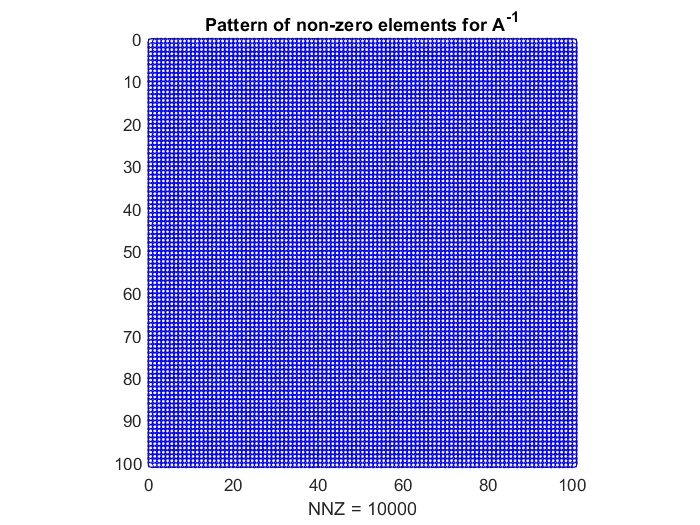
\includegraphics[width=.55\textwidth]{CG1_1e2_dense} &\hspace{-25pt} 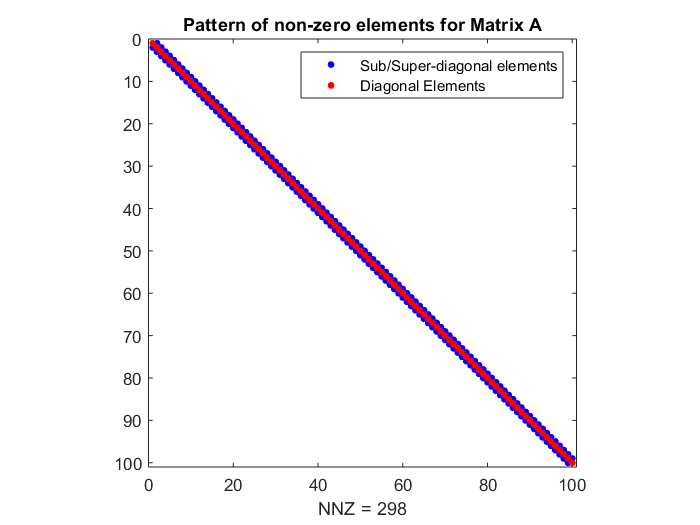
\includegraphics[width=.55\textwidth]{CG1_1e2_sparse} \\
		(a) & (b)\\
		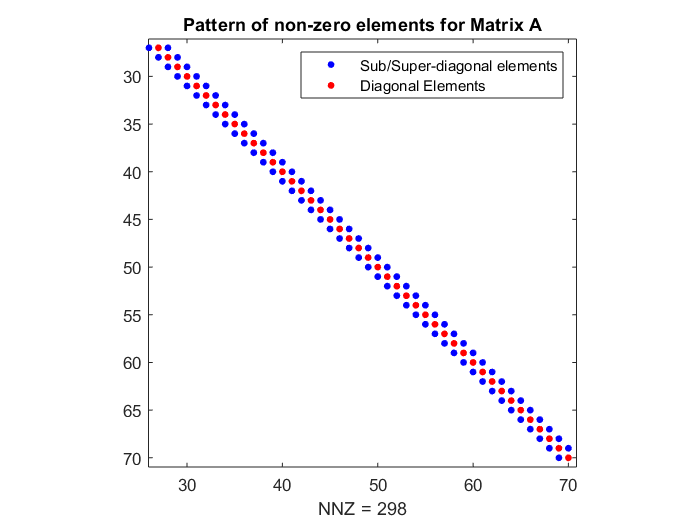
\includegraphics[width=.55\textwidth]{CG1_1e2_sparse_zoom} &\hspace{-25pt} 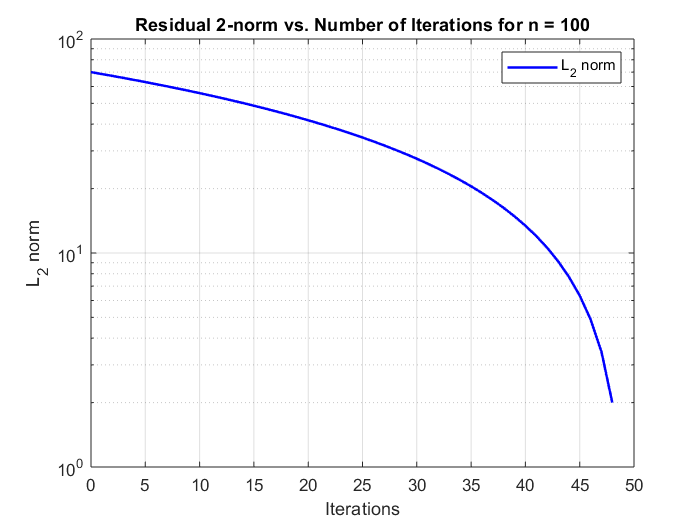
\includegraphics[width=.55\textwidth]{CG1_1e2_norm} \\
		c) & d)\\
	\end{tabular}
	\caption{$A^{-1}$ a), $A$ b) and its zoomed-in version c) and the Euclidean Norm of the residual as a function of the iterations d)}
	\label{}
\end{figure}

\begin{figure}[!ht]
	\centering
	\begin{tabular}{cc}
		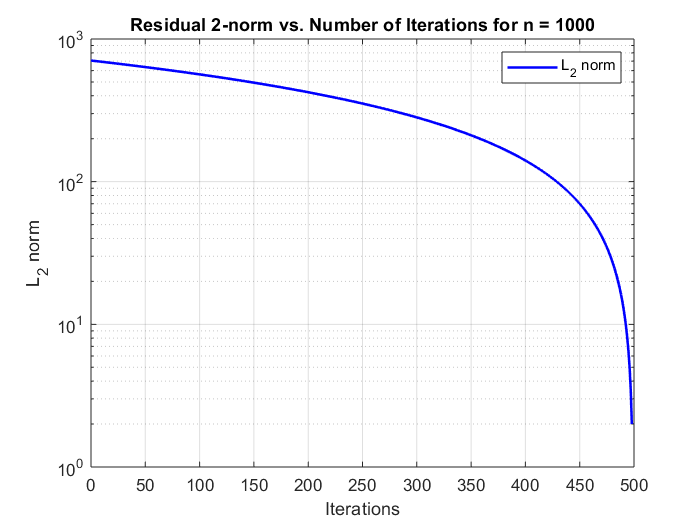
\includegraphics[width=.55\textwidth]{CG1_1e3_norm} &\hspace{-25pt} 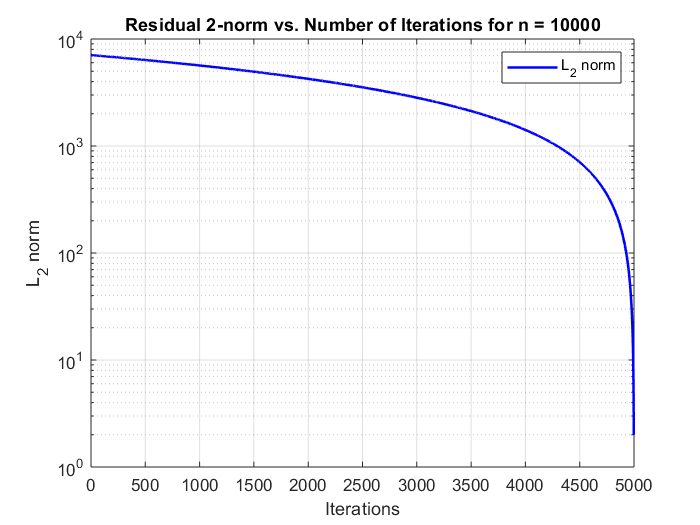
\includegraphics[width=.55\textwidth]{CG1_1e4_norm} \\
		(a) & (b)\\
	\end{tabular}
	\caption{Euclidean norm for the given values of $n$}
	\label{}
\end{figure}

\clearpage
For the 2-dimensional problem, we have
\begin{figure}[!ht]
	\centering
	\begin{tabular}{cc}
		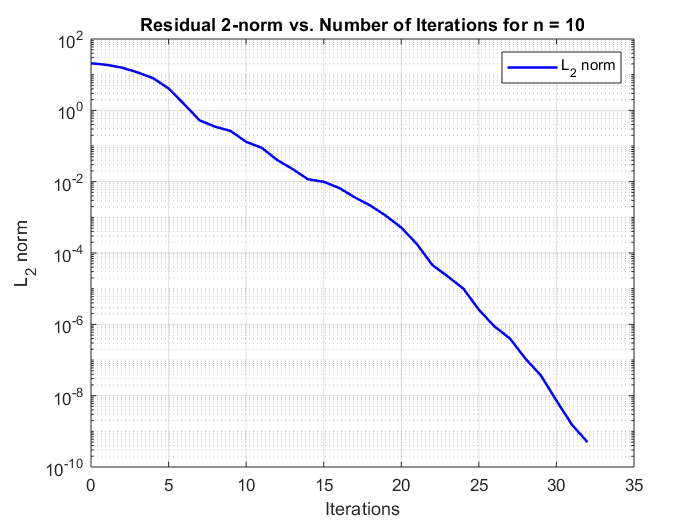
\includegraphics[width=.55\textwidth]{CG2_1e1_norm} &\hspace{-25pt} 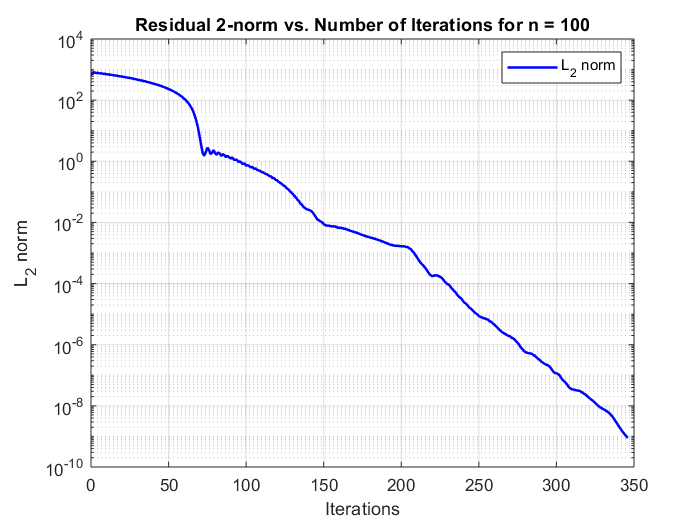
\includegraphics[width=.55\textwidth]{CG2_1e2_norm} \\
		(a) & (b)\\
	\end{tabular}
	\caption{Euclidean norm for the given values of $n$}
	\label{}
\end{figure}

For the 3-dimensional problem, we have:
\begin{figure}[!ht]
	\centering
		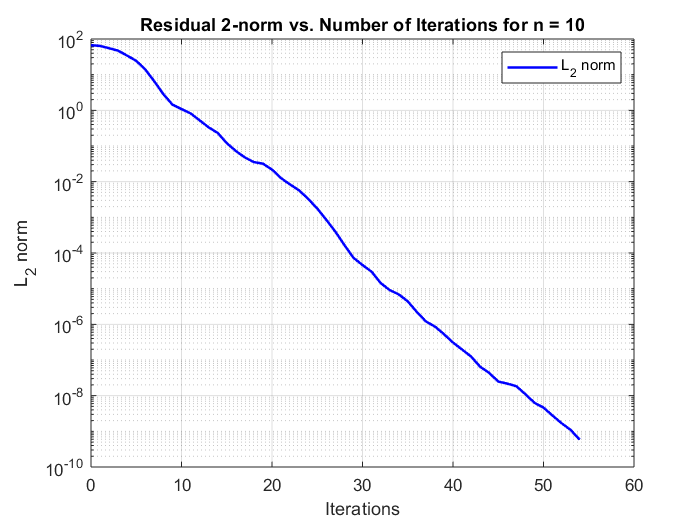
\includegraphics[width=.55\textwidth]{CG3_1e1_norm} \hspace{-25pt}
	\caption{Euclidean norm for the given values of $n$}
	\label{}
\end{figure}

\clearpage
\section*{Problem 2}
For this problem we use the Conjugate Gradient Algorithm to solve the system $A{\bf x}={\bf b}$, where $A$ is the Hilbert Matrix. We summarize our result below.

\begin{center}
	\begin{tabular}{||c | c | c | c|||} 
		\hline
		n & Elapsed Time & Iterations (sec) & Condition Number\\ [0.5ex] 
		\hline\hline
		5 & 0.0087 & 6 & 4.8$\times{10^{5}}$\\ 
		\hline
		8 & 0.0051 & 19 & 1.5$\times{10^{10}}$\\
		\hline
		12 & 0.0117 & 35 & 1.9$\times{10^{16}}$\\
		\hline
		20 & 0.0201 & 66 & 2.5$\times{10^{16}}$\\
		\hline
	\end{tabular}
\end{center}

\begin{figure}[!ht]
	\centering
	\begin{tabular}{cc}
		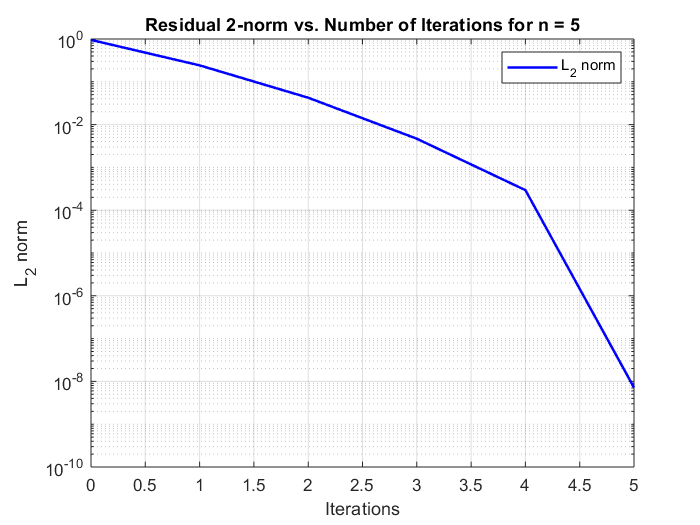
\includegraphics[width=.55\textwidth]{Hillbert_norm_n5} &\hspace{-25pt} 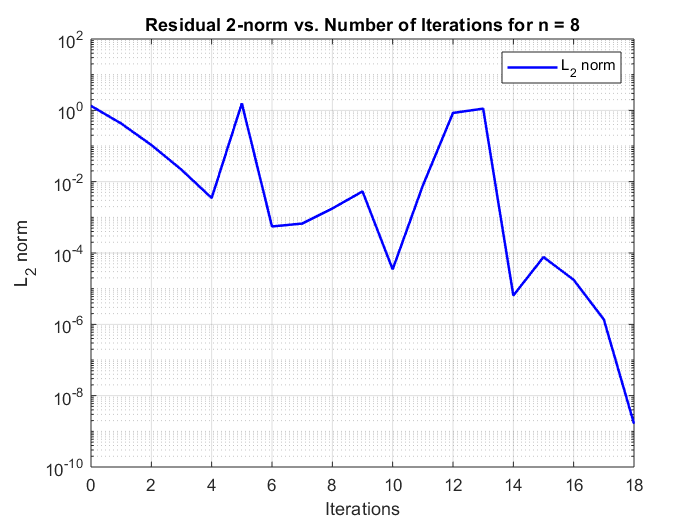
\includegraphics[width=.55\textwidth]{Hillbert_norm_n8} \\
		(a) & (b)\\
		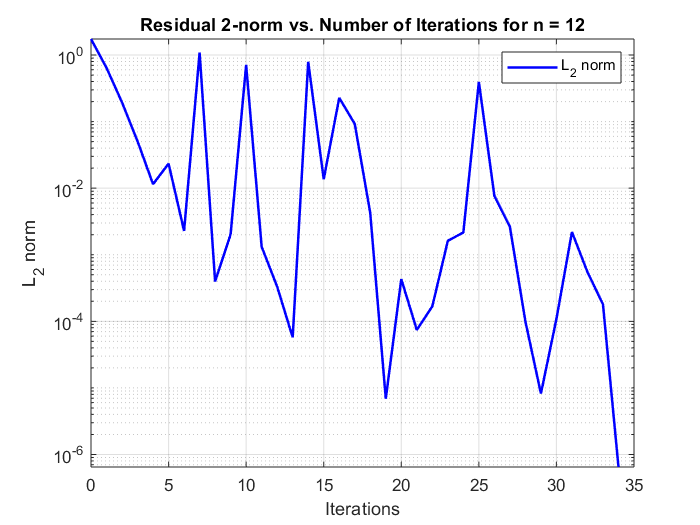
\includegraphics[width=.55\textwidth]{Hillbert_norm_n12} &\hspace{-25pt} 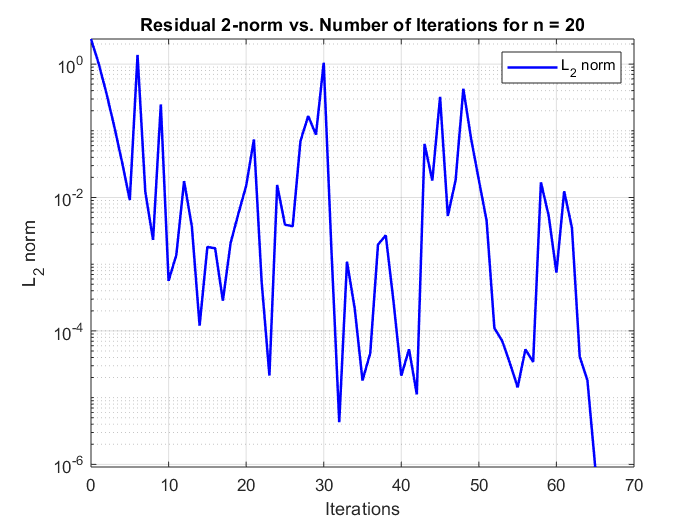
\includegraphics[width=.55\textwidth]{Hillbert_norm_n20} \\
		c) & d)\\
	\end{tabular}
	\caption{Residual Euclidean Norm as a function of the iterations for the given values of n}
	\label{}
\end{figure}
\clearpage

\begin{figure}[!ht]
	\centering
	\begin{tabular}{cc}
		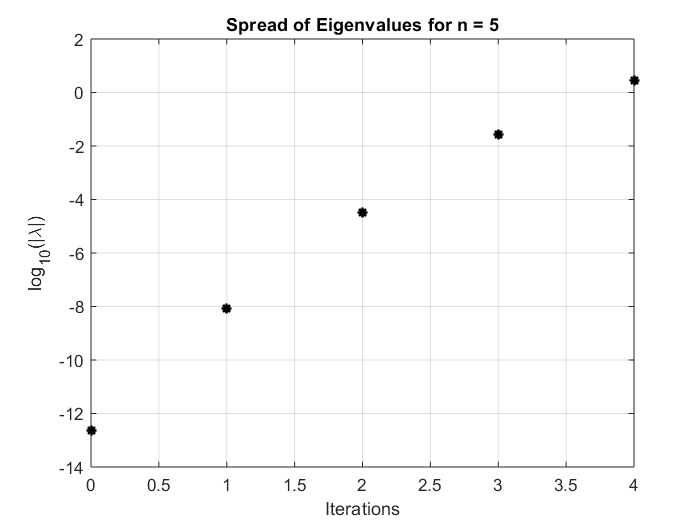
\includegraphics[width=.55\textwidth]{Hillbert_eig_n5} &\hspace{-25pt} 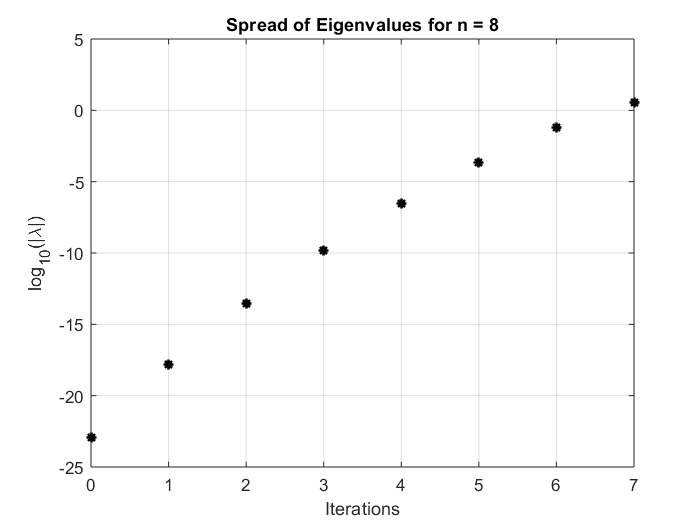
\includegraphics[width=.55\textwidth]{Hillbert_eig_n8} \\
		(a) & (b)\\
		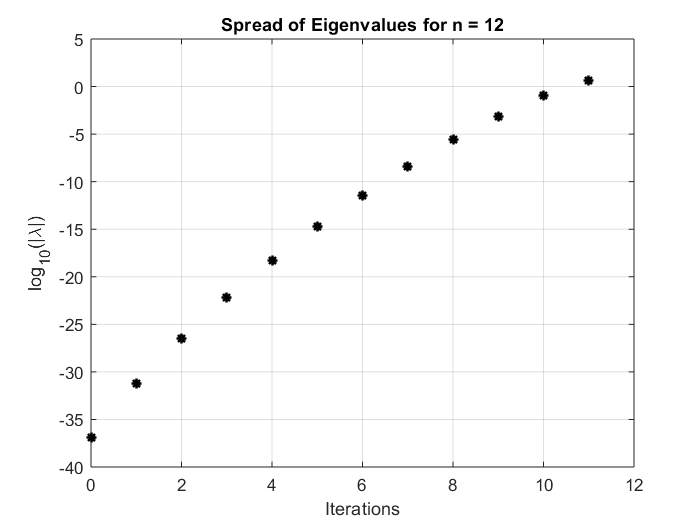
\includegraphics[width=.55\textwidth]{Hillbert_eig_n12} &\hspace{-25pt} 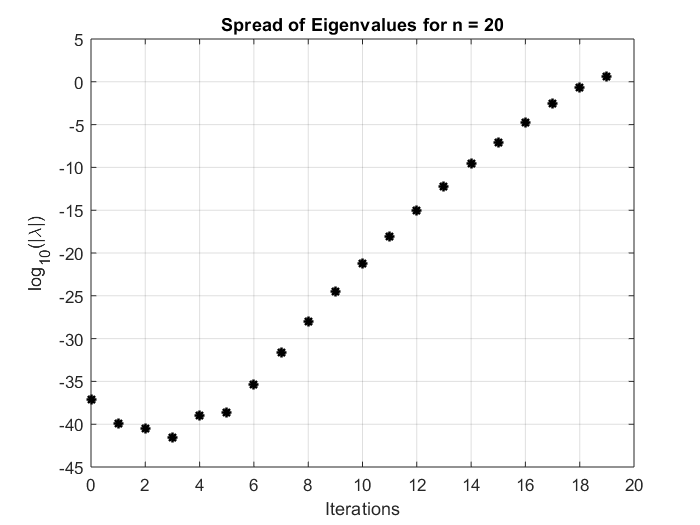
\includegraphics[width=.55\textwidth]{Hillbert_eig_n20} \\
		c) & d)\\
	\end{tabular}
	\caption{Spread of the Eigenvalues of the Hilbert Matrix for dimensions $n=5$ a), $n=8$ b), $n=12$ c) and $n=20$ d)}
	\label{}
\end{figure}

\clearpage
\section*{Appendix - Matlab Code}
\subsection*{Codes for Problem 1}
\subsubsection*{One-dimensional}
\lstinputlisting{CG.m}
\clearpage
\subsubsection*{Two-dimensional}
\lstinputlisting{CG2.m}
\clearpage
\subsubsection*{Three-dimensional}
\lstinputlisting{CG3.m}
\clearpage
\subsection*{Code for Problem 2}
\lstinputlisting{Hillbert.m}
\end{document}